%!TEX TS-program = xelatex
%!TEX encoding = UTF-8 Unicode
% Awesome CV LaTeX Template for CV/Resume
%
% This template has been downloaded from:
% https://github.com/posquit0/Awesome-CV
%
% Author:
% Claud D. Park <posquit0.bj@gmail.com>
% http://www.posquit0.com
%
%
% Adapted to be an Rmarkdown template by Mitchell O'Hara-Wild
% 23 November 2018
%
% Template license:
% CC BY-SA 4.0 (https://creativecommons.org/licenses/by-sa/4.0/)
%
%-------------------------------------------------------------------------------
% CONFIGURATIONS
%-------------------------------------------------------------------------------
% A4 paper size by default, use 'letterpaper' for US letter
\documentclass[11pt, a4paper]{awesome-cv}

% Configure page margins with geometry
\geometry{left=1.4cm, top=.8cm, right=1.4cm, bottom=1.8cm, footskip=.5cm}

% Specify the location of the included fonts
\fontdir[fonts/]

% Color for highlights
% Awesome Colors: awesome-emerald, awesome-skyblue, awesome-red, awesome-pink, awesome-orange
%                 awesome-nephritis, awesome-concrete, awesome-darknight

\colorlet{awesome}{awesome-red}

% Colors for text
% Uncomment if you would like to specify your own color
% \definecolor{darktext}{HTML}{414141}
% \definecolor{text}{HTML}{333333}
% \definecolor{graytext}{HTML}{5D5D5D}
% \definecolor{lighttext}{HTML}{999999}

% Set false if you don't want to highlight section with awesome color
\setbool{acvSectionColorHighlight}{true}

% If you would like to change the social information separator from a pipe (|) to something else
\renewcommand{\acvHeaderSocialSep}{\quad\textbar\quad}

\def\endfirstpage{\newpage}

%-------------------------------------------------------------------------------
%	PERSONAL INFORMATION
%	Comment any of the lines below if they are not required
%-------------------------------------------------------------------------------
% Available options: circle|rectangle,edge/noedge,left/right

\name{Deependra}{Dhakal}

\address{Siranchowk-3 (Harmi), Gorkha}

\mobile{+977 9845333283}
\email{\href{mailto:ddhakal.rookie@gmail.com}{\nolinkurl{ddhakal.rookie@gmail.com}}}
\homepage{rookie.rbind.io}
\github{deependrad}
\twitter{dd\_rookie}

% \gitlab{gitlab-id}
% \stackoverflow{SO-id}{SO-name}
% \skype{skype-id}
% \reddit{reddit-id}


\usepackage{booktabs}

\providecommand{\tightlist}{%
	\setlength{\itemsep}{0pt}\setlength{\parskip}{0pt}}

%------------------------------------------------------------------------------


\usepackage{tabularx}

\newcommand{\recommendation}[6]{% change this to accept more details
  \noindent
  \begin{tabularx}{.5\linewidth}{@{\extracolsep{2pt}} l p{5cm} }
    Name: & \bfseries\textit{#1} \\
    Designation: & #2 \\
    Department: & #3 \\
    Institute: & #4 \\
    Mobile: & #5 \\
    Email: & #6 % \\
    % Other: & #7
  \end{tabularx}%
}

% \graphicspath{{cv/}}
\newcommand{\bpicture}{\begin{picture}(0,0)\put(460,50)}
\newcommand{\epicture}{\end{picture}}

\usepackage{multicol}

\newcommand{\bmulticols}{\begin{multicols}{2}}
\newcommand{\emulticols}{\end{multicols}}

% Pandoc CSL macros
\newlength{\cslhangindent}
\setlength{\cslhangindent}{1.5em}
\newlength{\csllabelwidth}
\setlength{\csllabelwidth}{3em}
\newenvironment{CSLReferences}[3] % #1 hanging-ident, #2 entry spacing
 {% don't indent paragraphs
  \setlength{\parindent}{0pt}
  % turn on hanging indent if param 1 is 1
  \ifodd #1 \everypar{\setlength{\hangindent}{\cslhangindent}}\ignorespaces\fi
  % set entry spacing
  \ifnum #2 > 0
  \setlength{\parskip}{#2\baselineskip}
  \fi
 }%
 {}
\usepackage{calc}
\newcommand{\CSLBlock}[1]{#1\hfill\break}
\newcommand{\CSLLeftMargin}[1]{\parbox[t]{\csllabelwidth}{#1}}
\newcommand{\CSLRightInline}[1]{\parbox[t]{\linewidth - \csllabelwidth}{#1}}
\newcommand{\CSLIndent}[1]{\hspace{\cslhangindent}#1}

\begin{document}

% Print the header with above personal informations
% Give optional argument to change alignment(C: center, L: left, R: right)
\makecvheader

% Print the footer with 3 arguments(<left>, <center>, <right>)
% Leave any of these blank if they are not needed
% 2019-02-14 Chris Umphlett - add flexibility to the document name in footer, rather than have it be static Curriculum Vitae
\makecvfooter
  {March 2021}
    {Deependra Dhakal~~~·~~~Curriculum Vitae}
  {\thepage}


%-------------------------------------------------------------------------------
%	CV/RESUME CONTENT
%	Each section is imported separately, open each file in turn to modify content
%------------------------------------------------------------------------------



\bpicture

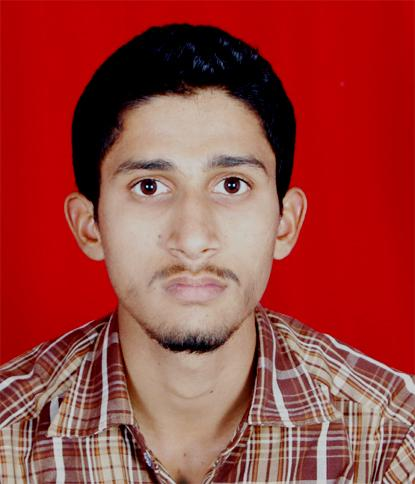
\includegraphics[width=5em]{Photo_pp.jpg} \epicture

\hypertarget{education}{%
\section{Education}\label{education}}

\begin{cventries}
    \cventry{Agriculture and Forestry Campus, Rampur}{Agriculture and Forestry University}{Chitwan}{2016--2018}{\begin{cvitems}
\item First Division
\end{cvitems}}
    \cventry{Institute of Agriculture and Animal Science}{Tribhuvan University}{Lamjung}{2010--2015}{\begin{cvitems}
\item First Division
\end{cvitems}}
    \cventry{Orchid Science College}{Higher Secondary Education Board}{Chitwan}{2008--2010}{\begin{cvitems}
\item First Division
\end{cvitems}}
    \cventry{Small Heaven Higher Secondary Boarding School}{SLC Board}{Chitwan}{2008}{\begin{cvitems}
\item Distinction
\end{cvitems}}
\end{cventries}

\hypertarget{competencies}{%
\section{Competencies}\label{competencies}}

\hypertarget{computing}{%
\subsection{Computing}\label{computing}}

\hypertarget{scripting}{%
\subsubsection*{Scripting}\label{scripting}}
\addcontentsline{toc}{subsubsection}{Scripting}

\begin{multicols}{2}
\begin{itemize}
\item Python, 
\item R, 
\item Bash,
\item Javascript,
\item Markdown,
\item \LaTeX,
\item HTML
\end{itemize}
\end{multicols}

\hypertarget{domain-applications}{%
\subsubsection*{Domain applications}\label{domain-applications}}
\addcontentsline{toc}{subsubsection}{Domain applications}

\begin{multicols}{2}
\begin{itemize}
\item Crop modeling
\item DSSAT
\item GIS and spatial analysis
\item QGIS
\end{itemize}
\end{multicols}

\hypertarget{general-purpose-applications}{%
\subsubsection*{General purpose
applications}\label{general-purpose-applications}}
\addcontentsline{toc}{subsubsection}{General purpose applications}

\begin{multicols}{2}
\begin{itemize}
\item ImageMagick,
\item Tesseract,
\item MS Word, MS Excel, VBscript,
\item Adobe Photoshop
\end{itemize}
\end{multicols}

\hypertarget{communication-language}{%
\subsection{Communication Language}\label{communication-language}}

\begin{itemize}
\tightlist
\item
  Nepali
\item
  Hindi
\item
  English
\end{itemize}

\hypertarget{training-and-experience}{%
\section{Training and Experience}\label{training-and-experience}}

\begin{cventries}
    \cventry{Department of Plant Breeding and Genetics}{Gokuleshwor Agriculture and Animal Science College}{Baitadi, Nepal}{March 29 2019--Ongoing}{\begin{cvitems}
\item \textit{Assistant Professor}
\end{cvitems}}
    \cventry{Crop Breeding and Research Division}{Unique Seed Company Pvt. Ltd.}{Dhangadhi, Kailali, Nepal}{May 9, 2018--March 28, 2019}{\begin{cvitems}
\item \textit{Crop Breeder}
\end{cvitems}}
    \cventry{representing Unique Seed Company Pvt. Ltd.}{National training workshop on 'Seed Quality and Productivity Enhancement Technologies in Lentil'; Organized by: CIMMYT and NGLRP/NARC}{Nepalgunj, Nepal}{February 17, 2019--February 18, 2019}{}\vspace{-4.0mm}
    \cventry{representing Unique Seed Company Pvt. Ltd.}{International training workshop on 'Hybrid Vegetable Seed Production and Marketing'; Organized by: HRD/NARC, SEAN, CIMMYT and World Vegetable Center}{Dang, Nepal}{February 13, 2019--February 15, 2019}{}\vspace{-4.0mm}
    \cventry{representing Unique Seed Company Pvt. Ltd.}{International training on "Hybrid Maize Seed Production and Marketing"; Organized by: CIMMYT}{Kathmandu, Nepal}{October 1, 2018--October 3, 2018}{}\vspace{-4.0mm}
    \cventry{representing Unique Seed Company Pvt. Ltd.}{International training on "Statistical Data Analysis"; Organized by: CIMMYT}{Kathmandu, Nepal}{September 29, 2018--September 30, 2018}{}\vspace{-4.0mm}
    \cventry{representing Unique Seed Company Pvt. Ltd.}{International training on 'Hybrid Maize Comprehensive Technologies'; Organized by: Yuan Longping High-Tech Agriculture Co. Ltd., Changsha, China and NMRP/NARC, Nepal}{Chitwan, Nepal}{July 17, 2018--August 31, 2018}{}\vspace{-4.0mm}
    \cventry{FORWARD Nepal}{Enhancing quality standards of raw milk: Validation of Good Manufacturing Practices(GMP) in the supply chain.}{Tanahun, Nepal}{November 2016--December 2016}{\begin{cvitems}
\item \textit{Field Research Associate}
\end{cvitems}}
    \cventry{Nepal Development Research Institute}{Action Research for Cost Effective Agricultural Extension Services in 10 mid-hill districts of Nepal.}{Rukum, Nepal}{March 2014--April 2014}{\begin{cvitems}
\item \textit{Enumerator}
\end{cvitems}}
\end{cventries}

\hypertarget{research-interests}{%
\section{Research interests}\label{research-interests}}

\begin{cvhonors}
    \cvhonor{}{Interested in Mathematical modeling}{Cropping systems simulation and inference on ecological data}{}
    \cvhonor{}{Interested in Geo-spatial statistics}{Feature identification and visual summary of data}{}
    \cvhonor{}{Interested in Multivariate analysis}{of genotype and phenotype information}{}
    \cvhonor{}{Interested in Design and optimization of experiments}{Both for controlled environments and without environmental control; Randomization based design and design search algorithms}{}
\end{cvhonors}

\newpage

\hypertarget{publications}{%
\section{Publications}\label{publications}}

\hypertarget{bibliography}{}
\leavevmode\hypertarget{ref-paudel2020archives}{}%
1. Paudel, S., \& Dhakal, D. (2020). Archives of agriculture and
environmental science. \emph{Archives of Agriculture and Environmental
Science}, \emph{5}(2), 190--195.
\url{https://doi.org/10.26832/24566632.2020.0502016}

\leavevmode\hypertarget{ref-kalauni2020correlation}{}%
2. Kalauni, S., \& Dhakal, D. (2020). Correlation and path coefficient
analysis of seed yield and yield components of french bean (phaseolus
vulgaris l.) genotypes in sub-tropical region. \emph{Turkish Journal of
Agriculture-Food Science and Technology}, \emph{8}(9), 1928--1934.
\url{https://doi.org/10.24925/turjaf.v8i9.1928-1934.3528}

\leavevmode\hypertarget{ref-ddhakal-agro-morpho2015:iaasproceeding-lamjung}{}%
3. Dhakal, D., \& Subedi, R. (2015). Study of agro-morphological
descriptors of common bean (phaseolus vulgaris l.) genotypes. In B. D.
Regmi (Ed.), \emph{Proceedings of undergraduate practicum assessment
volume 2} (pp. 23--26). IAAS.

\leavevmode\hypertarget{ref-ddhakal2018postanthesis}{}%
4. Deependra, D. (2018). \emph{Post-anthesis leaf health as potential
determinant of yield in early evaluation trial of wheat genotypes} {[}MS
Thesis{]}. Agriculture~and~Forestry~University.

\leavevmode\hypertarget{ref-iaasproceeding-lamjung}{}%
5. Regmi, B. D. (Ed.). (2015). \emph{Proceedings of undergraduate
practicum assessment volume 2}. IAAS.

\hypertarget{advisor-and-referee}{%
\section{Advisor and Referee}\label{advisor-and-referee}}

\bmulticols

\columnbreak

\hypertarget{dr.-madhav-prasad-pandey}{%
\subsubsection*{Dr.~Madhav Prasad
Pandey}\label{dr.-madhav-prasad-pandey}}
\addcontentsline{toc}{subsubsection}{Dr.~Madhav Prasad Pandey}

\begin{itemize}
\tightlist
\item
  Professor
\item
  Department of Genetics and Plant Breeding
\item
  Agriculture and Forestry University
\item
  9855081410
\item
  \href{mailto:mppandey@afu.edu.np}{mppandey@afu.edu.np}
\end{itemize}

\hypertarget{dr.-krishna-hari-dhakal}{%
\subsubsection*{Dr.~Krishna Hari Dhakal}\label{dr.-krishna-hari-dhakal}}
\addcontentsline{toc}{subsubsection}{Dr.~Krishna Hari Dhakal}

\begin{itemize}
\tightlist
\item
  Chairman
\item
  Department of Genetics and Plant Breeding
\item
  Agriculture and Forestry University
\item
  9843561486
\item
  \href{mailto:khdhakal@afu.edu.np}{khdhakal@afu.edu.np}
\end{itemize}

\columnbreak

\hypertarget{mr.-laxmi-kant-dhakal}{%
\subsubsection*{Mr.~Laxmi Kant Dhakal}\label{mr.-laxmi-kant-dhakal}}
\addcontentsline{toc}{subsubsection}{Mr.~Laxmi Kant Dhakal}

\begin{itemize}
\tightlist
\item
  Chairman
\item
  Unique Seed Company Pvt. Ltd.
\item
  Dhangadhi, Kailali
\item
  9858420560
\item
  \href{mailto:krishak14@gmail.com}{krishak14@gmail.com}
\end{itemize}

\emulticols

\vspace{1.5cm}
\parbox[t]{\textwidth}{
{\bfseries Declaration}\par

I hereby declare that, all the information stated above is true and genuine in my belief. I can dispense any and/or all of the mentioned works in verified form whenever demanded.
}

\end{document}
